\documentclass[12pt,draftclsnofoot,onecolumn]{IEEEtran}

\usepackage{comment,url}
\usepackage[dvips]{graphicx}
\usepackage{caption,subfig}
\usepackage{float}
\graphicspath{{../fig/}}
\DeclareGraphicsExtensions{.eps}
\usepackage{setspace}
\usepackage{amsmath}
\usepackage{amssymb}
\usepackage{cite}
\hyphenation{op-tical net-works semi-conduc-tor}

\usepackage{array}
\usepackage{mdwmath}
\usepackage{mdwtab}
\newtheorem{thm}{Theorem}
\doublespacing

\begin{document}

\title{On the Distribution of Random\\Distances in Rhombuses}

\author{Yanyan Zhuang~$^{\dagger *}$ and T. Aaron Gulliver~$^\ddagger$\\
$^\dagger$~University of British Columbia, Vancouver, BC, Canada\\
$^*$~NYU Polytechnic, New York, NY, USA\\
$^\ddagger$~University of Victoria, Victoria, BC, Canada}

\maketitle
\thispagestyle{empty}

\begin{abstract}
The distribution of random distances in geometric figures has important
applications in probability, statistics and many applied fields.
The study of the distribution of random distances in rhombuses is presented
in this work. Results are derived using an approach which is easier to
employ than previous results in the literature. Explicit
probability density functions are presented which are useful in a wide range of applied
areas such as operations research and wireless communications.
\end{abstract}

\section{Introduction}
Rhombuses are one of the basic building blocks in two-dimensional tilings. The
distance distributions related to rhombuses have practical applications in a
wide range of fields, including urban transportation, operations research, and wireless communications.
Different from rectangles and squares, the point coordinates in rhombuses are
not independent. This paper presents a new and simpler analytic approach which can be used
to handle the dependency among point coordinates in rhombuses. This new approach
is an improvement of the author's prior work in~\cite{zhuang2011random}
and~\cite{zhuang2012geometrical}. The results for rhombuses are extended
to obtain similar results for regular hexagons, which
are widely used in planar tessellations in cellular
networks~\cite{zhuang2011geometric}, wireless ad-hoc
networks~\cite{zhuang2013planar}, and wireless sensor
networks~\cite{schwiebert2001research, chang2008hexagonal, wang2009analytical},
and many general wireless networking applications~\cite{baltzis2012distance}.

In this work, results are derived for the distribution of
the random Euclidean distances within the same rhombus, between two parallel rhombuses
sharing a side, and between two rhombuses sharing a common diagonal.
% The approach used is easier to interpret than our prior
% work~\cite{zhuang2011random, zhuang2012geometrical}

\section{From Square to Rhombus}
For a rectangle with sides of lengths $a$ and $b$, define $X=x_1-x_2$,
$Y=y_1-y_2$, where $(x_1, y_1)$ and $(x_2, y_2)$ are the coordinates of two
random points in the rectangle. Assuming $x_1, x_2 \in [0,a]$ and $y_1, y_2 \in
[0, b]$ are uniformly and independently distributed, $X$ and $Y$ have the following
distributions
\begin{equation}\label{eq:fxy}
  f_X(x)=\frac{1}{a^2}\left\{
    \begin{array}{lr}
      a+x & -a\leq x \leq 0 \\
      a-x & 0 \leq x \leq a
    \end{array}
  \right.
  % \end{equation}
  % and
  % \begin{equation}
  ~~\mbox{ and }~~ f_Y(y)=\frac{1}{b^2}\left\{
    \begin{array}{lr}
      b+y & -b\leq y \leq 0 \\
      b-y & 0 \leq y \leq b
    \end{array}
  \right..
\end{equation}
%
Note that the distributions of $X$ and $Y$ are independent. The
distance between $(x_1, y_1)$ and $(x_2, y_2)$ is $D=\sqrt{X^2+Y^2}$. Let the
squared distance be $Z=D^2=X^2+Y^2$, then
\begin{eqnarray}\label{eq-rec}
F_Z(z)&=&\iint F_{Z|X=x, Y=y}(z)f_{X,Y}(x,y){\rm d}x{\rm d}y\nonumber\\
&=&\iint F\left(X^2+Y^2 \leq z\right|X=x, Y=y)f_{X,Y}(x,y){\rm d}x{\rm
d}y\nonumber\\
&=&\iint_{\Omega_{X^2+Y^2 \leq z}}f_{X,Y}(x,y){\rm d}x{\rm d}y=
\iint_{\Omega_{X^2+Y^2 \leq z}}f_X(x)f_Y(y){\rm d}x{\rm d}y
\end{eqnarray}
where $X^2+Y^2 \leq z$ is the interior of a circle with radius $\sqrt{z}$, and
$\Omega_{X^2+Y^2 \leq z}$ is the region where both $X^2+Y^2 \leq z$ and
$f_X(x)f_Y(y)$ are non-zero. The last equality in (\ref{eq-rec}) holds because
$X$ and $Y$ are independent in a rectangle.

Note that the region $\Omega_{X^2+Y^2 \leq z}$ is critical. It expresses the
random variable $Z$ as a function of two other independent random variables
$Z=X^2+Y^2$, and characterizes the distribution of $Z$, $P(Z\leq z)$, through
$X$ and $Y$. The region $\Omega_{X^2+Y^2 \leq z}$ is therefore a projection
of the surface of $X^2+Y^2 \leq z$, as $z$ varies, onto the
$X$-$Y$ space where $f_X(x)f_Y(y)$ is non-zero.
Such an interpretation is similar to that in~\cite{ghosh1943distribution, ghosh1943random}
where the distance distributions for rectangles were derived.
Note that the formulation in (\ref{eq-rec}) improves on the results
in~\cite{zhuang2011random, zhuang2012geometrical} in that it simplifies the analysis.
As a special case, if $(x_1, y_1)$ and $(x_2, y_2)$ are located
in a unit square, then
\begin{equation}\label{eq:fxy-sqr}
  f_X(x)=\left\{
    \begin{array}{lr}
      1+x & -1\leq x \leq 0 \\
      1-x & 0 \leq x \leq 1
    \end{array}
  \right.
  % \end{equation}
  % and
  % \begin{equation}
  ~~\mbox{ and }~~ f_Y(y)=\left\{
    \begin{array}{lr}
      1+y & -1\leq y \leq 0 \\
      1-y & 0 \leq y \leq 1
    \end{array}
  \right..
\end{equation}

Since a circle is symmetric with respect to both $X$ and $Y$, the
distribution of $Z$ is four times the distribution in the first quadrant, giving
% where $0 \leq x \leq 1$ and $0 \leq y \leq 1$,
\begin{equation}\label{eq:f_z1}
F_Z(z)=4\iint_{\Omega}(1-x)(1-y){\rm d}x{\rm d}y,
\end{equation}
where $\Omega$ is the interior of the circle $X^2+Y^2 \leq z$ when $0 \leq X \leq 1$
and $0 \leq Y \leq 1$.
This is a much more general form than the expressions in~\cite{zhuang2011random,
zhuang2012geometrical}, and thus is more useful and easier to derive new results.
%use and  can only express (\ref{eq:f_z1}) in explicit form.
Similarly, in the next section (\ref{eq:within}), (\ref{eq:para}), (\ref{eq:fz_longdiag}) and
(\ref{eq:fz_shortdiag}) are easily obtained using the general expression in (\ref{eq-rho}).
With $D=\sqrt{Z}$, the distance probability density function is
\begin{equation}\label{eq:fd-fz}
f_D(d)=F_Z'(d^2)=2df_Z(d^2).
\end{equation}

\section{Distribution of Random Distances in a Rhombus}

\begin{figure}
  \centering
  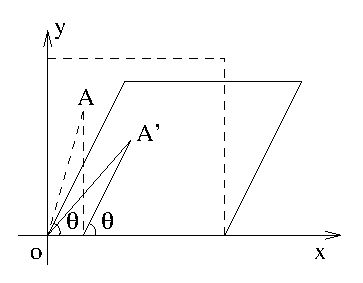
\includegraphics[width=0.4\columnwidth]{fig/single_rhombus}
  \caption{Random points in a rhombus.}
  \label{fig:rhombus}
\end{figure}

From Figure~\ref{fig:rhombus}, there is a linear relationship between a point $A
(x,y)$ in a square, and a point $A' (x',y')$ in a rhombus given by
\begin{equation}\label{eq:xr}
 \left\{
\begin{array}{lc}
x'=x+y\cos \theta \\
y'=y \sin \theta
\end{array}
\right.,
\end{equation}
where $\theta$ is the acute angle of the rhombus. In the following, we
assume both sides of the rhombus in Figure~\ref{fig:rhombus} are of unit
length and $\theta=\frac{\pi}{3}$, so that $x'=x+\frac{y}{2}$ and $y'=\frac{\sqrt{3}y}{2}$.

\begin{figure}
  \centering
  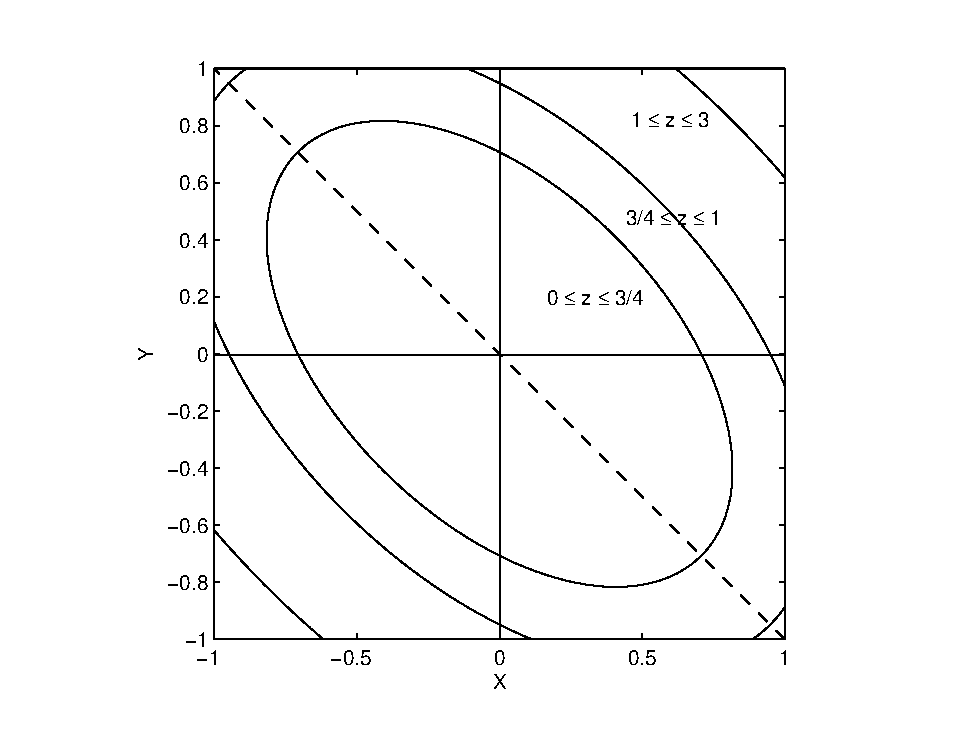
\includegraphics[width=0.5\columnwidth]{fig/rhombus_within}
  \caption{Ellipse $X^2+XY+Y^2 \leq z$ for the random distances in a rhombus.}
  \label{fig:z1}
\end{figure}

For two random points in a rhombus $(x_1',y_1')$ and $(x_2',y_2')$, define
$X'=x_1'-x_2'=\left(x_1-x_2\right)+\frac{1}{2}\left(y_1-y_2\right)=X+\frac{1}{2}
Y$, and
$Y'=y_1'-y_2'=\frac{\sqrt{3}}{2}\left(y_1-y_2\right)=\frac{\sqrt{3}}{2}Y$, where
$(x_1, y_1)$ and $(x_2, y_2)$ are the coordinates of two random points in a
unit square. $X$ and $Y$ have the same distribution as in
(\ref{eq:fxy-sqr}). The squared distance is $Z=D^2=X'^2+Y'^2=\left(X+\frac{1}{2}
Y\right)^2+\left(\frac{\sqrt{3}}{2}Y\right)^2=X^2+XY+Y^2$. Similar to
(\ref{eq-rec}), we have
\begin{eqnarray}\label{eq-rho}
F_Z(z)&=&\iint F\left(X^2+XY+Y^2 \leq z\right|X=x, Y=y)f_{X,Y}(x,y){\rm d}x{\rm
d}y\nonumber\\
&=&\iint_{\Omega_{X^2+XY+Y^2 \leq z}}f_{X,Y}(x,y){\rm d}x{\rm d}y=
\iint_{\Omega_{X^2+XY+Y^2 \leq z}}f_X(x)f_Y(y){\rm d}x{\rm d}y,
\end{eqnarray}
where $X^2+XY+Y^2 \leq z$ is the interior of an ellipse with semi-major axis
equal to $\sqrt{2z}$, and semi-minor axis equal to $\sqrt{\frac{2z}{3}}$.
$\Omega_{X^2+XY+Y^2 \leq z}$ is the region where both $X^2+XY+Y^2 \leq z$ and
$f_X(x)f_Y(y)$ are non-zero. In the following, the subscript of $\Omega$ is
omitted when it is clear from the context.
Note that the formulation in (\ref{eq-rho}) is much simpler than that given in~\cite{zhuang2011random}
and~\cite{zhuang2012geometrical}.

From Figure~\ref{fig:z1}, ellipse $X^2+XY+Y^2 \leq z$ is symmetric with respect
to $Y=-X$ and $Y=X$. The distribution of $Z$ is therefore
\begin{equation}\label{eq:within}
F_Z(z)=2\left[\iint_{\Omega_1}(1-x)(1-y){\rm d}x{\rm
d}y+\iint_{\Omega_2}(1-x)(1+y){\rm d}x{\rm d}y\right],
\end{equation}
where $\Omega_1$ is the interior of ellipse $X^2+XY+Y^2 \leq z$ with $0 \leq X
\leq 1$ and $0 \leq Y \leq 1$; and $\Omega_2$ is the interior of this ellipse with
$0 \leq X \leq 1$ and $-1 \leq Y \leq 0$. As an example in Figure~\ref{fig:z1},
when $0\leq z \leq \frac{3}{4}$, $F_Z(z)$ can be derived as
\begin{small}
\begin{eqnarray}\label{eq:Z1_r_within}
F_Z(z)&=&2\left[\int_{0}^{\sqrt{z}}\int_{0}^{-\frac{y}{2}+\sqrt{z-\frac{3}{4}y^2
}}(1-x){\rm d}x(1-y){\rm
d}y+2\int_{-\sqrt{z}}^0\int_{-y}^{-\frac{y}{2}+\sqrt{z-\frac{3}{4}
y^2}}(1-x){\rm d}x(1+y){\rm d}y\right] \nonumber\\
&=&\left(\frac{2}{3}+\frac{\pi}{9\sqrt{3}}\right)z^2-\frac{32}{9}z^{3/2}+\frac{
2\pi}{\sqrt{3}}z.
\end{eqnarray}
\end{small}%
Similarly, the case when $\frac{3}{4} \leq z \leq 1$ and $1 \leq z \leq 3$ can
be derived according to (\ref{eq:within}). Note that in~\cite{zhuang2011random}
and~\cite{zhuang2012geometrical}, (\ref{eq:Z1_r_within}) was derived directly
for this particular case, which is a much more complex approach than via the
more useful and general expression given in (\ref{eq:within}). Using (\ref{eq:fd-fz}), the
probability density function of the random distances between two uniformly
distributed points that are both inside the same rhombus is then
\begin{small}
 \begin{equation}\label{eq:fd_r_within}
  f_{D_{\rm I}}(d)=2d\left\{
    \begin{array}{lr}

\left(\frac{4}{3}+\frac{2\pi}{9\sqrt{3}}\right)d^2-\frac{16}{3}d+\frac{2\pi}{
\sqrt{3}} & 0\leq d\leq \frac{\sqrt{3}}{2}\\

\frac{8}{\sqrt{3}}\left(1+\frac{d^2}{3}\right)\sin^{-1}\frac{\sqrt{3}}{2d}
+\left(\frac{4}{3}-\frac{10\pi}{9\sqrt{3}}\right)d^2-\frac{16}{3}d+\frac{10}{3}
\sqrt{4d^2-3}-\frac{2\pi}{\sqrt{3}} & \frac{\sqrt{3}}{2}\leq d\leq 1\\

\frac{4}{\sqrt{3}}\left(1-\frac{d^2}{3}\right)\sin^{-1}\frac{\sqrt{3}}{2d}
-\left(\frac{2}{3}-\frac{2\pi}{9\sqrt{3}}\right)d^2+\sqrt{4d^2-3}-\frac{2\pi}{
3\sqrt{3}}-1 & 1\leq d\leq \sqrt{3} \\

      0 & {\rm otherwise}
    \end{array}
  \right..
\end{equation}
\end{small}
This result was obtained in~\cite{zhuang2011random} and~\cite{zhuang2012geometrical} using
a much more complex approach.

\section{Distribution of Random Distances between Two Rhombuses}

\begin{figure}
  \centering
  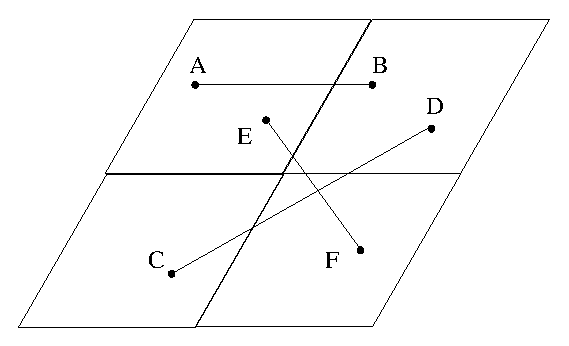
\includegraphics[width=0.4\columnwidth]{fig/rhombus}
  \caption{Random Points in Two Rhombuses.}
  \label{fig:two}
\end{figure}

In addition to two points in the same rhombus, we have i) two parallel rhombuses
sharing a side, i.e., random distance $AB$ in Figure~\ref{fig:two}, ii) two
rhombuses sharing a common diagonal, such as $CD$ and $EF$. Here $CD$ and $EF$
are two different cases, and in the following, we refer them as long diagonal
(long-diag) and short diagonal (short-diag), respectively.

\subsection{Distribution of Random Distances between Two Parallel Rhombuses Sharing a
Side}

\begin{figure}
  \centering
  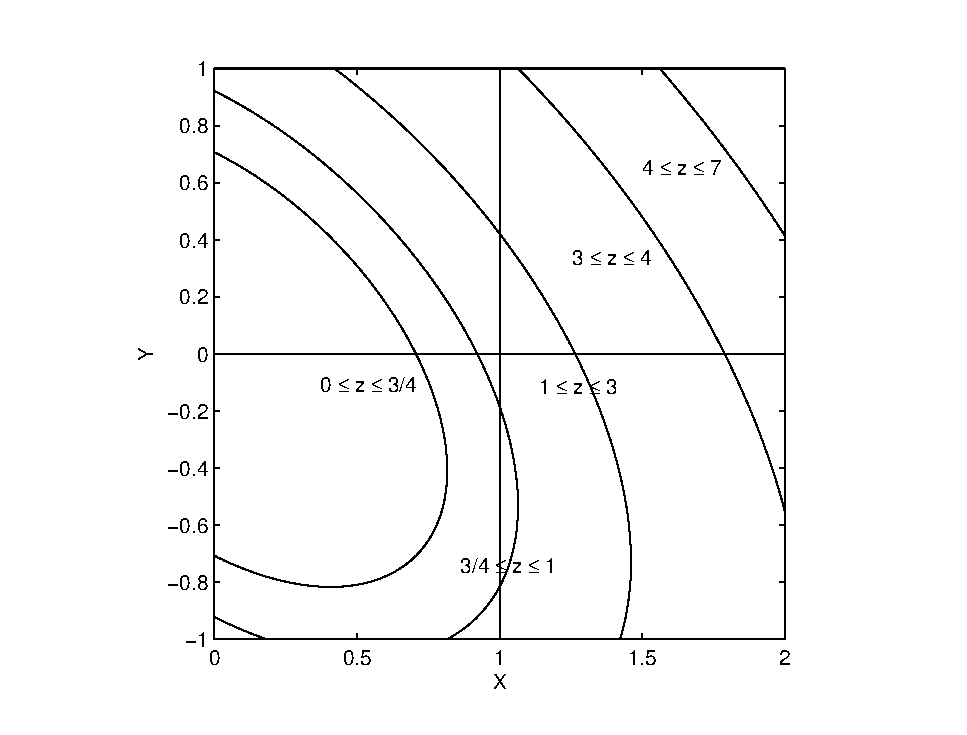
\includegraphics[width=0.5\columnwidth]{fig/rhombus_para}
  \caption{Ellipse $X^2+XY+Y^2 \leq z$ for random distances between two parallel rhombuses sharing a side.}
  \label{fig:para}
\end{figure}

For $AB$ in Figure~\ref{fig:two}, the distributions of $X$ and $Y$ are
\begin{equation}\label{eq:fxy_para}
  f_X(x)=\left\{
    \begin{array}{lr}
      x & 0\leq x \leq 1 \\
      2-x & 1 \leq x \leq 2
    \end{array}
  \right.,
  ~~\mbox{ and }~~ f_Y(y)=\left\{
    \begin{array}{lr}
      1+y & -1\leq y \leq 0 \\
      1-y & 0 \leq y \leq 1
    \end{array}
  \right.,
\end{equation}
respectively.
The distribution of $Z$ is the same as in (\ref{eq-rho}), with
$f_X(x)$ and $f_Y(y)$ as above. The ellipse $X^2+XY+Y^2 \leq z$
is shown in Figure~\ref{fig:para}. This gives
\begin{eqnarray}\label{eq:para}
 F_Z(z)&=&\iint_{\Omega_1}x(1+y){\rm d}x{\rm d}y+\iint_{\Omega_2}x(1-y){\rm
d}x{\rm d}y\nonumber \\
&&+\iint_{\Omega_3}(2-x)(1+y){\rm d}x{\rm d}y+\iint_{\Omega_4}(2-x)(1-y){\rm
d}x{\rm d}y,
\end{eqnarray}
where $\Omega_1$ is the interior of ellipse $X^2+XY+Y^2 \leq z$ with $0 \leq X
\leq 1$ and $-1 \leq Y \leq 0$; $\Omega_2$ is the interior of this ellipse
with $0 \leq X \leq 1$, $0 \leq Y \leq 1$; and $\Omega_3$ and $\Omega_4$ exist only when
$1 \leq X \leq 2$ and $-1 \leq Y \leq 0$, and $1 \leq X \leq 2$ and $0 \leq Y
\leq 1$, respectively.
% where $\Omega_1$ to $\Omega_4$ are the interior of ellipse $X^2+XY+Y^2 \leq z$
% in four different quadrants, respectively.
As shown in Figure~\ref{fig:para}, depending on the value of $z$, not all four regions
$\Omega_1$ to $\Omega_4$ exist in (\ref{eq:para}). For example, when $0\leq z
\leq \frac{3}{4}$, $\Omega_3$ and $\Omega_4$ do not exist. $F_Z(z)$ in this case is
\begin{small}
\begin{eqnarray}\label{eq:Z1_r_para}
 F_Z(z)&=&\left[\int_0^{\sqrt{\frac{4z}{3}}}\int_{-\frac{x}{2}-\sqrt{z-\frac{3}{
4}x^2}}^{-\sqrt{\frac{z}{3}}}(1+y){\rm d}yx{\rm d}x+\int_{-\sqrt{\frac{z}{3}}}
^0\int_0^{-\frac{y}{2}+\sqrt{z-\frac{3}{4}y^2}}x{\rm d}x(1+y){\rm d}y\right]
\nonumber\\
&&+\int_0^{\sqrt{z}}\int_0^{-\frac{y}{2}+\sqrt{z-\frac{3}{4}y^2}}
x{\rm d}x(1-y){\rm
d}y=\frac{8}{9}z^{3/2}-\left(\frac{1}{3}+\frac{\pi}{18\sqrt{3}}
\right)z^2.
\end{eqnarray}
\end{small}
Note that in~\cite{zhuang2011random}
and~\cite{zhuang2012geometrical}, (\ref{eq:Z1_r_para}) was derived directly for just this particular case.
This is more difficult than employing the more general expression given in (\ref{eq:para}).
Using an approach similar to that above with (\ref{eq:fd-fz}), the probability density
function of the random distances between two uniformly distributed points, one
in each of the two adjacent rhombuses that are parallel and sharing a side is
\begin{small}
 \begin{equation}\label{eq:fd_r_para}
  f_{D_{\rm P}}(d)=2d\left\{
    \begin{array}{lr}

\frac{4}{3}d-\left(\frac{2}{3}+\frac{\pi}{9\sqrt{3}}\right)d^2 & 0\leq d\leq
\frac{\sqrt{3}}{2}\\

-\frac{2}{\sqrt{3}}(d^2+2)\sin^{-1}\frac{\sqrt{3}}{2d}+\left(\frac{8\pi}
{9\sqrt{3}}-\frac{2}{3}\right)d^2+\frac{4}{3}d-\frac{11}{6}\sqrt{4d^2-3}+\frac{
2\pi}{\sqrt{3}} & \frac{\sqrt{3}}{2}\leq d\leq 1\\

\frac{4d^2}{3\sqrt{3}}\sin^{-1}\frac{\sqrt{3}}{2d}+\left(\frac{2}{3}
-\frac{2\pi}{9\sqrt{3}}\right)d^2-\frac{8}{3}d+\frac{\sqrt{4d^2-3}}{3}+\frac{
2\pi}{3\sqrt{3}}+\frac{1}{2} & 1\leq d\leq \sqrt{3} \\

\left(\frac{2}{\sqrt{3}}-\frac{d^2}{3\sqrt{3}}\right)\sin^{-1}\frac{\sqrt
{3}}{2d}+\left(\frac{2}{\sqrt{3}}+\frac{d^2}{3\sqrt{3}}\right)\sin^{-1}\frac{
\sqrt{3}}{d}+\left(\frac{1}{3}-\frac{\pi}{9\sqrt{3}}\right)d^2 \\
~~~~-\frac{8}{3}d+\frac{7}{12}\sqrt{4d^2-3}+\sqrt{d^2-3}+\frac{3}{4}
-\frac{2\pi}{3\sqrt{3}} & \sqrt{3}\leq d\leq 2 \\

\left(\frac{2}{\sqrt{3}}-\frac{d^2}{3\sqrt{3}}\right)\left(\sin^{-1}\frac{
\sqrt{3}}{2d}+\sin^{-1}\frac{\sqrt{3}}{d}\right)+\left(\frac{\pi}{9\sqrt{3}}
-\frac{1}{3 }\right)d^2 \\
~~~~+\frac{7}{12}\sqrt{4d^2-3}+\frac{\sqrt{d^2-3}}{3}-\frac{2\pi}{3\sqrt{3}}
-\frac{5}{4} & 2 \leq d \leq \sqrt{7} \\

      0 & {\rm otherwise}
    \end{array}
 \right..
\end{equation}
\end{small}

\subsection{Distribution of Random Distances between Two Long-Diag Rhombuses}

\begin{figure}
  \centering
  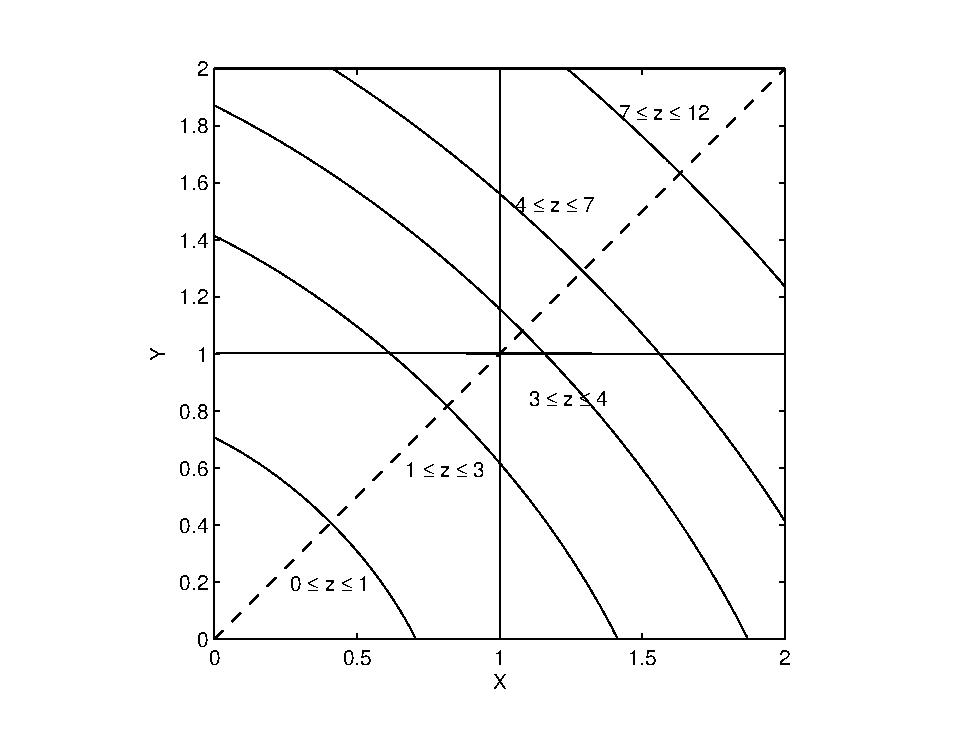
\includegraphics[width=0.5\columnwidth]{fig/rhombus_diag1}
  \caption{Ellipse $X^2+XY+Y^2 \leq z$ for random distances between two long-diag rhombuses.}
  \label{fig:diag1}
\end{figure}

For $CD$ in Figure~\ref{fig:two}, the distributions of $X$ and $Y$ are
\begin{equation}\label{eq:fxy_diag}
  f_X(x)=\left\{
    \begin{array}{lr}
      x & 0\leq x \leq 1 \\
      2-x & 1 \leq x \leq 2
    \end{array}
  \right.,
  ~~\mbox{ and }~~ f_Y(y)=\left\{
    \begin{array}{lr}
      y & 0\leq y \leq 1 \\
      2-y & 1 \leq y \leq 2
    \end{array}
  \right.,
\end{equation}
respectively.
The ellipse $X^2+XY+Y^2 \leq z$ is shown in Figure~\ref{fig:diag1}. As this
ellipse is symmetric with respect to $Y=X$, the distribution of $Z$ is
\begin{equation}\label{eq:fz_longdiag}
 F_Z(z)=\iint_{\Omega_1}xy{\rm d}x{\rm d}y+2\iint_{\Omega_2}x(2-y){\rm d}x{\rm
d}y+\iint_{\Omega_3}(2-x)(2-y){\rm d}x{\rm d}y,
\end{equation}
where $\Omega_1$ is the interior of ellipse $X^2+XY+Y^2 \leq z$ with $0 \leq X
\leq 1$ and $0 \leq Y \leq 1$; $\Omega_2$ is the interior of this ellipse with
$0 \leq X \leq 1$ and $1 \leq Y \leq 2$; and $\Omega_3$ exists only when $1 \leq X \leq 2$
and $1 \leq Y \leq 2$.
For example, when $0\leq z \leq 1$, only $\Omega_1$
exists, so that
\begin{small}
 \begin{equation}
 F_Z(z)=\int_0^{\sqrt{z}}\int_0^{-\frac{y}{2}+\sqrt{z-\frac{3}{4}y^2}}
x{\rm d}xy{\rm d}y=\left(\frac{1}{6}-\frac{\pi}{18\sqrt{3}}\right)z^2.
\end{equation}
\end{small}

Therefore, the probability density function of the random distances between two
uniformly distributed points, one in each of the two adjacent rhombuses sharing
a common long diagonal is
\begin{small}
\begin{equation}\label{eq:fd_r_diag1}
  f_{D_{\rm LD}}(d)=2d\left\{
    \begin{array}{lr}

\left(\frac{1}{3}-\frac{\pi}{9\sqrt{3}}\right)d^2 & 0\leq d\leq 1\\

-\frac{4d^2}{3\sqrt{3}}\sin^{-1}\frac{\sqrt{3}}{2d}+\left(\frac{\pi}{3\sqrt{3}}
-1\right)d^2+\frac{8}{3}d-\frac{\sqrt{4d^2-3}}{3}-1 & 1\leq d\leq \sqrt{3}\\

\frac{4}{\sqrt{3}}\left(\frac{d^2}{3}-2\right)\sin^{-1}\frac{\sqrt{3
}}{2d}+\left(\frac{1}{3}-\frac{\pi}{9\sqrt{3}}\right)d^2+\frac{8}{3}d-\frac{7}{3
}\sqrt{4d^2-3}+\frac{4\pi}{3\sqrt{3}}+1 & \sqrt{3}\leq d\leq 2\\

\frac{4}{\sqrt{3}}\left(\frac{d^2}{3}-2\right)\sin^{-1}\frac{\sqrt{3
}}{2d}+\frac{2d^2}{3\sqrt{3}}\sin^{-1}\frac{\sqrt{3}}{d}+\left(1-\frac{\pi}{
3\sqrt{3}}\right)d^2 \\
~~~~-\frac{7}{3}\sqrt{4d^2-3}+\frac{2}{3}\sqrt{d^2-3}+\frac{4\pi}{3\sqrt{3}}+3 &
2\leq d\leq \sqrt{7} \\

\frac{2}{\sqrt{3}}\left(4-\frac{d^2}{3}\right)\sin^{-1}\frac{\sqrt{3}}{d}
+\left(\frac{\pi}{9\sqrt{3}}-\frac{1}{3}\right)d^2+2\sqrt{d^2-3}-\frac{4\pi}{
3\sqrt{3}}-2 & \sqrt{7} \leq d \leq 2\sqrt{3} \\

      0 & {\rm otherwise}
    \end{array}
  \right..
\end{equation}
\end{small}

\subsection{Distribution of Random Distances between Two Short-Diag Rhombuses}

\begin{figure}
  \centering
  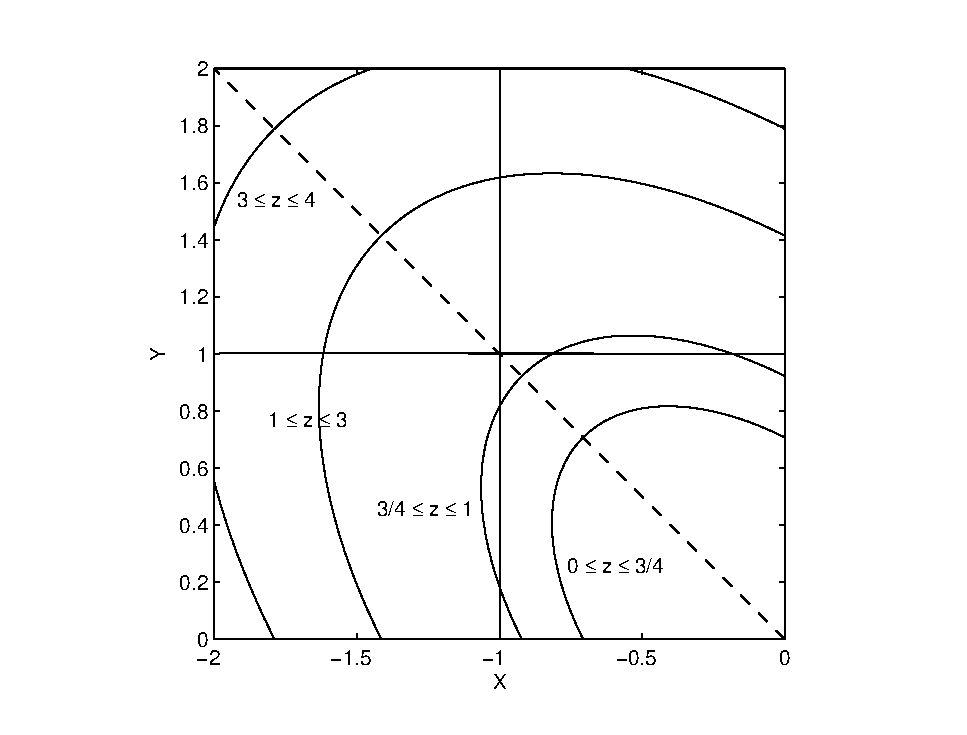
\includegraphics[width=0.5\columnwidth]{fig/rhombus_diag2}
  \caption{Ellipse $X^2+XY+Y^2 \leq z$ for random distances between two short-diag rhombuses.}
  \label{fig:diag2}
\end{figure}

For $EF$ in Figure~\ref{fig:two}, the distributions of $X$ and $Y$ are
\begin{equation}
  f_X(x)=\left\{
    \begin{array}{lr}
      2+x & -2\leq x \leq -1 \\
      -x & -1 \leq x \leq 0
    \end{array}
  \right.,
  ~~\mbox{ and }~~ f_Y(y)=\left\{
    \begin{array}{lr}
      y & 0\leq y \leq 1 \\
      2-y & 1 \leq y \leq 2
    \end{array}
  \right.,
\end{equation}
respectively.
The ellipse $X^2+XY+Y^2 \leq z$ is shown in Figure~\ref{fig:diag2}. As the
ellipse is symmetric with respect to $Y=-X$, the distribution of $Z$ is
\begin{equation}\label{eq:fz_shortdiag}
 F_Z(z)=\iint_{\Omega_1}(-x)y{\rm d}x{\rm d}y+2\iint_{\Omega_2}(-x)(2-y){\rm
d}x{\rm d}y+\iint_{\Omega_3}(2+x)(2-y){\rm d}x{\rm d}y,
\end{equation}
where $\Omega_1$ is the interior of ellipse $X^2+XY+Y^2 \leq z$ with $-1 \leq X
\leq 0$ and $0 \leq Y \leq 1$; $\Omega_2$ is the interior of this ellipse with
$-1 \leq X \leq 0$ and $1 \leq Y \leq 2$; and $\Omega_3$ exists only when $-2 \leq X \leq
-1$ and $1 \leq Y \leq 2$.
For example, when $\frac{3}{4} \leq z \leq 1$,
$\Omega_3$ does not exist so the distribution of $Z$ is
\begin{small}
 \begin{eqnarray}\label{eq:Z2_r_diag2}
 F_Z(z)&=&\left[2\int_{-\sqrt{z}}^0\int_{-x}^{-\frac{x}{2}+\sqrt{z-\frac{3}{4}
x^2}}y{\rm d}y(-x){\rm
d}x-2\int_{-\frac{1}{2}-\sqrt{z-\frac{3}{4}}}^{-\frac{1}{2}+\sqrt{
z-\frac{3}{4}}}\int_1^{-\frac{x}{2}+\sqrt{z-\frac{3}{4}x^2}}y{\rm d}y(-x){\rm
d}x\right] \nonumber\\
&&+2\int_{-\frac{1}{2}-\sqrt{z-\frac{3}{4}}}^{-\frac{1}{2}+\sqrt{z-\frac{3}{4}}}
\int_1^{-\frac{x}{2}+\sqrt{z-\frac{3}{4}x^2}}(2-y){\rm d}y(-x){\rm d}x
\nonumber\\
&=&-\frac{2z^2}{3\sqrt{3}}\sin^{-1}\frac{\sqrt{3}}{2}\frac{\sqrt{4z-3}}{z}
+\left(\frac{1}{6}+\frac{\pi}{9\sqrt{3}}\right)z^2+\frac{10z-3}{18}\sqrt{4z-3}.
\end{eqnarray}
\end{small}

The probability density function of the random distances between two uniformly
distributed points, one in each of the two adjacent rhombuses sharing a common
short diagonal is
\begin{small}
\begin{equation}\label{eq:fd_r_diag2}
  f_{D_{\rm SD}}(d)=2d\left\{
    \begin{array}{lr}

\left(\frac{1}{3}+\frac{2\pi}{9\sqrt{3}}\right)d^2 & 0\leq d\leq
\frac{\sqrt{3}}{2}\\

\frac{8d^2}{3\sqrt{3}}\sin^{-1}\frac{\sqrt{3}}{2d}+\left(\frac{1}{3}-\frac{10\pi
}{9\sqrt{3}}\right)d^2+\frac{2}{3}\sqrt{4d^2-3} & \frac{\sqrt{3}}{2} \leq d \leq
1\\

-\left(\frac{4d^2}{3\sqrt{3}}+\frac{8}{\sqrt{3}}\right)\sin^{-1}\frac{\sqrt{3}}{
2d}+\left(\frac{1}{3}+\frac{2\pi}{9\sqrt{3}}\right)d^2+\frac{8}{3}d-3\sqrt{
4d^2-3}+\frac{8\pi}{3\sqrt{3}}+1 & 1\leq d\leq \sqrt{3} \\

\frac{8}{\sqrt{3}}\sin^{-1}\frac{\sqrt{3}}{d}-d^2+\frac{8}{3}d+\frac{8}{3}\sqrt{
d^2-3}-\frac{8\pi}{3\sqrt{3}}-4 & \sqrt{3}\leq d\leq 2 \\

      0 & {\rm otherwise}
    \end{array}
  \right..
\end{equation}
\end{small}

Equations (\ref{eq:fd_r_para}), (\ref{eq:fd_r_diag1}) and
(\ref{eq:fd_r_diag2}) were derived in~\cite{zhuang2011random}
and~\cite{zhuang2012geometrical} using a more complex approach.
However, the intermediate results given in (\ref{eq:within}), (\ref{eq:para}),
(\ref{eq:fz_longdiag}) and (\ref{eq:fz_shortdiag}) are easily obtained using (\ref{eq-rho}).

\section{Conclusion}
This paper considered the distribution of random distances in geometric figures,
in particular rhombuses.
New results were presented using a new approach which is easier to
employ than previous results in the literature.
Explicit probability density functions were presented.
These results have applications in probability, statistics and applied fields
such as operations research and wireless communications.

\section*{Acknowledgement}
Yanyan Zhuang would like to acknowledge the guidance she received related to the
subject matter presented in this work from 2010 to 2011 at the University of
Victoria.

\bibliographystyle{IEEEtran}
\bibliography{bibdata}

\end{document} 